\documentclass[12pt,fleqn]{article}\usepackage{../../common}
\begin{document}
Ders 27

Uclu entegralleri gorduk, pek cok kordinat sisteminde bu hesaplari
yapabiliyoruz. Simdi vektor alanlarini isleyecegiz, ozellikle akis (flux)
ve is (work) kavramlarina bakacagiz. 

Uzayda Vektor Alanlari

Vektor alani demek, her noktada bir vektor olmasi demek, bu vektorun
her ogesinin $x,y,z$ kordinatlarina bagli olmasi demek. Alan $\vec{F}$
icin mesela 

$$
\vec{F} = < P,Q,R >
$$

olabilir ve $P,Q,R$ birer fonksiyondur, $P(x,y,z)$ gibi. 

Ornekler

a)

Mesela kuvvet alanlari, yercekim kuvveti gibi, belli bir noktada belli
bir yone bir kuvvet etkisi var, bu bir kuvvet alani, vektor alani olarak
gosterilebilir. Yercekim alani orijin (0,0,0)'a dogru olan bir cekim kuvveti
olsun, ve buyuklugu $\frac{c}{\rho^2}$ gibi bir sabite oranli olsun, ki
$\rho$ orijine olan uzaklik. Kabaca bir resimde gosterirsek,

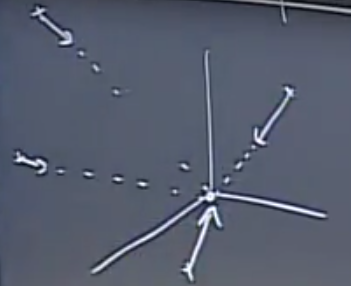
\includegraphics[width=20em]{calc_multi_27_01.png}

Goruldugu gibi cekim (ok) orijine dogru ve vektor buyuklugu (cekim kuvveti)
uzaklik arttikca kuculuyor. Birkac vektor cizdik sadece fikir vermesi
icin. Formulle belirtmek gerekirse,

$$
\vec{F} = \frac{-c < x,y,z >}{\rho^2}
$$

$< x,y,z >$'nin negatifi alindi, $< x,y,z >$ vektoru orijinden $x,y,z$'ye giden
vektor, oradan geri isaret eden vektor bunun negatif olurdu. Buyuklugu ise
$-c / \rho^2$ ile carparak ayarliyoruz. 

Benzer ornekler cogaltilabilir, elektrik alanlari, manyetik alanlar, vs.

b) 

Hiz alanlari bir diger ornek. Mesela sivi akisini temsil etmek istiyorsak,
ya da atmosferdeki ruzgar akisini incelemek istiyorsak, bunlari birer hiz alani
olarak gosterilebilir.

c)

Gradyan alanlari

Bir fonksiyon $u = u(x,y,z)$'nin gradyani $\nabla u = < u_x, u_y, u_z >$
bir gradyan alani olusturur.

Tabii ustteki ornekleri cok kesin hatlarla birbirinden ayri gibi gormemek lazim,
mesela elektrik ya da yercekim alanlari elektrik ya da yercekimsel potansiyel
fonksiyonunun gradyan alanidir. Gradyan matematiksel bir teknik, pek cok
yerde karsimiza cikabiliyor.

Yani vektor alanlari faydali seyler, bunu gorduk. Onlarla ne yapacagiz?
Akis konusu ile baslayalim.

Akis (Flux)

Daha once akis kavramini iki boyutta gormustuk,

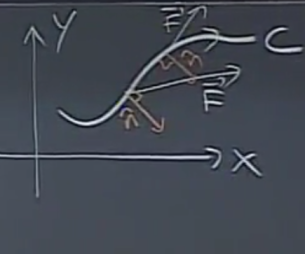
\includegraphics[width=10em]{calc_multi_27_02.png}

Bir vektor alani $\vec{F}$ icinde egri $C$ vardi, vektor alaninin
egriye dik olan bileseni ile bir akis entegrali olusturmustuk, bu
bir cizgi entegraliydi, formulu

$$
\int_C \vec{F} \cdot \hat{n} \ud s
$$

ki bu hesabin olctugu vektor alaninin ne kadar egri icinden / uzerinden
gectigiydi. Sivi mekaniginde mesela bu, bir hiz alani baglaminda, bize egri
uzerinden ne kadar sivi aktigini gosterebilirdi. Peki uc boyutta? Uc boyutta tek
egri uzerinden, mesela esen ruzgar, hesabi biraz anlamsiz olur. Bir egri yerine
bir yuzey uzerinden, icinden olan alan bileseni daha anlamli.

O zaman 3D icin bu entegrali degistirmek lazim, cizgi entegrali yerine yuzey
entegrali gerekiyor.  Yuzey iki boyutlu bir nesne, o sebeple cift entegral
kullanmamiz lazim, tabii bu entegrali dogru kurmamiz gerekiyor, bu yuzeyin
$x,y,z$ kordinatlari ile etkilesimi var, bir degiskenden kurtulmamiz lazim bir
sekilde ki cift entegral hesaplayabilelim, vs. Kavramsal olarak cizgi
entegraliyle paralellikler var, iki boyutta iki degisken vardi, egrinin ne
oldugu uzerinden bu degiskenler bire inmisti, burada uc degisken yuzey formulu
uzerinden ikiye indirgenecek.

3D akisi hesaplamak icin, $\vec{F}$ ve yuzey $S$ ile dusunursek (tek $\vec{F}$
vektoru aldatici olmasin her $x,y,z$ noktasinda bir $\vec{F}$ var), yuzeye
her noktada dik olan $\vec{F}$ bilesenini bulmamiz lazim, yani vektor alanimin
normal bileseni lazim, daha teknik belirtelim birim normal vektor $\hat{n}$.

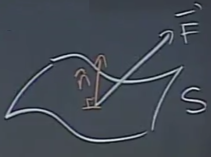
\includegraphics[width=10em]{calc_multi_27_03.png}

Normal vektor yonune karar vermek lazim once, resimde goruldugu gibi yukari, ya
da tam tersi asagi da alinabilir. Akis entegrallerinde bu karari vermek lazim,
yuzeyin bir tarafi secilmeli, ve oraya dogru giden vektor pozitif olarak
alinmali. Egri durumunda da bu tur bir secim yaptik, resme bakilirsa saga dogru,
saat yonu gidisi pozitif olarak aldik. Her durumda isleyen bir kural yok ama
eger bir bolge varsa orada disari ``cikan'' normaller daha iyi, o zaman bolgeden
disari cikisi olcmus oluyoruz.  Eger kapali bir yuzey yoksa genel olarak yukari
yonu secmek daha akilda kalir bir yontem olabilir.

Neyse yon secildikten sonra akis entegrali,

$$
\int \int_S \vec{F} \cdot \hat{n} \ud S
$$

$\ud S$ yuzey alan ufak parcasidir. Niye $\ud A$ kullanmadim, cunku bu
sembolu ileride kordinate yuzeyleri icin kullanmak istiyorum, daha once
cift entegrallerde gordugumuz gibi.

Akis hesabina gelelim, her ufak yuzey parcasi $\Delta S$ icin oradaki vektor
alani $\vec{F}$'nin yuzeye dik olan bilesenini hesapliyorum (o noktadaki
$\hat{n}$ ile carparak, bu bize $\vec{F}$'nin o noktadaki yuzeye dik bilesenini
verecektir), bu sonucu $\Delta S$ ile carpiyorum, ve bunu her parca icin
yaparak sonuclari topluyorum, cift entegral bu anlama geliyor.


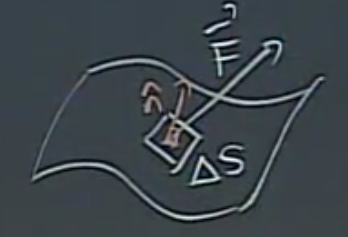
\includegraphics[width=15em]{calc_multi_27_04.png}

Not: Bazi kaynaklarda bazen $\ud \vec{S}$ gibi bir kullanim goruyorsunuz,
bu aslinda $\hat{n} \ud S$ demek oluyor. Vektor $ud \vec{S}$ yuzeye dik
olan ve buyuklugu ufak yuzey alanina tekabul eden bir vektordur. Niye
kullaniliyor? Daha az sembol yazmak icin degil sadece, bazen $ud \vec{S}$
hesabini yapmak ayri ayri $\hat{n}$ ve $\ud S$ kullanmaktan daha
kolay oluyor.

Ornek

$\vec{F} = < x,y,z >$ alaninin orijinde duran ve $a$ capli bir kure icinden
akisini hesaplayin.

Cevap

Soru oyle kurulmus ki cevap basit, cunku elde bir kure var, vektor alani
$< x,y,z >$, o zaman her noktada normal vektor ve vektor alani ayni yonu gosterir.

$$
\hat{n} = \frac{1}{a} < x,y,z >
$$

Ustteki birim vektor cunku $\sqrt{x^2 + y^2 + z^2} = a$.

Simdi $\vec{F} \cdot \hat{n}$'yi hesaplayalim, adim adim ilerliyoruz,
$\vec{F}$ her yerde $\hat{n}$ ile paralel oldugu icin
$\vec{F} \cdot \hat{n} = |\vec{F}| |\hat{n}| = |\vec{F}|$. Vektor $|\hat{n}|$
yokoldu cunku birim vektor, buyuklugu 1. Peki $|\vec{F}|$ nedir? Her
noktada bu deger $\sqrt{x^2 + y^2 + z^2}$ yani $a$. O zaman
$\vec{F} \cdot \hat{n} = a$.






















[devam edecek]

\end{document}
